\documentclass[tikz,border=5pt]{standalone}
\usepackage[UTF8]{ctex}
\usepackage{amsmath}
\usepackage[european resistors]{circuitikz}
\usetikzlibrary{arrows.meta,calc}
\definecolor{ink}{HTML}{243447}
\definecolor{blue}{HTML}{2765A2}
\definecolor{red}{HTML}{B74739}
\tikzset{line cap=round,line join=round,
vec/.style={thick,-{Latex[length=2mm]}},
every node/.style={font=\small}}
\newcommand{\ports}{
 \fill(0,3)circle(1.6pt)node[above left]{$A$};
 \fill(-2,0)circle(1.6pt)node[above left]{$B$};
 \fill(2,0)circle(1.6pt)node[above right]{$C$};
 \draw[blue,vec](0,4)--(0,3.15)node[midway,right]{$I_A$};
 \draw[blue,vec](-3.15,-.55)--(-2.15,-.07)node[pos=.2,above left]{$I_B$};
 \draw[blue,vec](2.15,-.07)--(3.15,-.55)node[pos=.8,above right]{$I_C$};
}
\newcommand{\network}{
 \draw(0,3)to[R,l_=$R$](-2,0);
 \draw(0,3)to[R,l=$R$](1,1.5)to[D](2,0);
 \draw(-2,0)to[R,l_=$R$](0,0)to[D](2,0);
}
\begin{document}
\begin{tikzpicture}
 \foreach \s/\reverse/\labeltext in {0/0/正向接入,3.65/1/反向接入}{
 \begin{scope}[xshift=\s cm]
  \ifnum\reverse=0
   \draw(0,1.6)to[D](1.3,1.6);
  \else
   \draw(1.3,1.6)to[D](0,1.6);
  \fi
  \draw(1.3,1.6)--(1.8,1.6);
  \draw(2.4,1.6)--(2.9,1.6)--(2.9,0)to[R,l_=$R$](1.05,0);
  \draw(2.1,1.6)circle(.3);
  \node at(2.1,1.6){$\mathrm{mA}$};
  \draw(1.05,0)--(.8,0);
  \draw(.55,-.36)--(.55,.36);
  \draw(.8,-.21)--(.8,.21);
  \draw(.55,0)--(0,0)--(0,1.6);
  \node[below]at(.55,-.37){$+$};
  \node[below]at(.8,-.37){$-$};
  \ifnum\reverse=0
   \draw[blue,vec](-.22,.35)--(-.22,1.15)node[midway,left]{$I_D$};
  \else
   \node[above]at(1.4,2){$I_D=0$};
  \fi
  \node at(1.45,-.95){\labeltext};
 \end{scope}
 }
 \begin{scope}[xshift=7.8cm,yshift=.05cm]
  \draw[gray,vec](-.65,0)--(3.05,0)node[right]{$U_D$};
  \draw[gray,vec](0,-.3)--(0,2.75)node[above]{$I_D$};
  \draw[blue,very thick](-.6,0)--(1.55,0)--(1.55,2.6);
  \node[below left]at(0,0){$O$};
  \node[below]at(1.55,-.04){$U_0=2\,\mathrm V$};
  \node at(1.25,-1){恒压降模型};
 \end{scope}
\end{tikzpicture}
\begin{tikzpicture}
 \foreach \s/\reverse/\labeltext in {0/0/{（a）正向为 $B\to C$},6.3/1/{（b）正向为 $C\to B$}}{
  \begin{scope}[xshift=\s cm]
   \draw(0,2.6)to[R,l_=$R_1$](-2,0);
   \draw(0,2.6)to[R,l=$R_2$](2,0);
   \ifnum\reverse=0
    \draw(-2,0)to[D](-.05,0);
   \else
    \draw(-.05,0)to[D](-2,0);
   \fi
   \draw(-.05,0)--(.55,0);
   \draw(1.15,0)--(2,0);
   \draw(.85,0)circle(.3);
   \node at(.85,0){$\mathrm{mA}$};
   \fill(0,2.6)circle(1.5pt)node[above left]{$A$};
   \fill(-2,0)circle(1.5pt)node[left]{$B$};
   \fill(2,0)circle(1.5pt)node[right]{$C$};
   \draw[blue,vec](0,3.65)--(0,2.75)node[midway,right]{$4\,\mathrm{mA}$};
   \draw[blue,vec](-2,-.15)--(-2,-1)node[midway,left]{$3\,\mathrm{mA}$};
   \draw[blue,vec](2,-.15)--(2,-1)node[midway,right]{$1\,\mathrm{mA}$};
   \node at(0,-1.5){\labeltext};
  \end{scope}
 }
\end{tikzpicture}
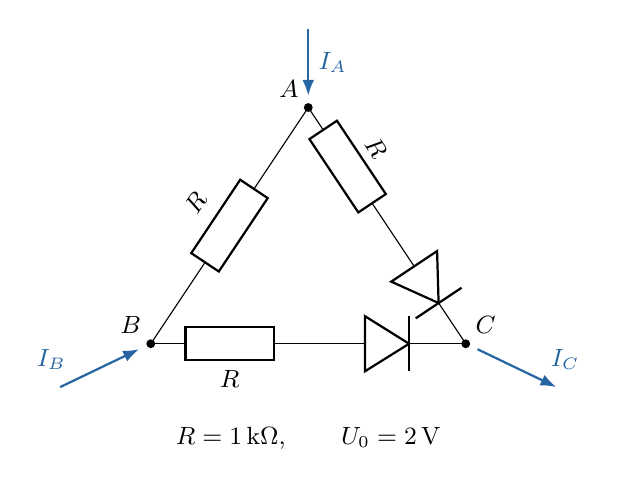
\begin{tikzpicture}
 \network
 \ports
 \node at(0,-1.2){$R=1\,\mathrm{k}\Omega,\qquad U_0=2\,\mathrm V$};
\end{tikzpicture}
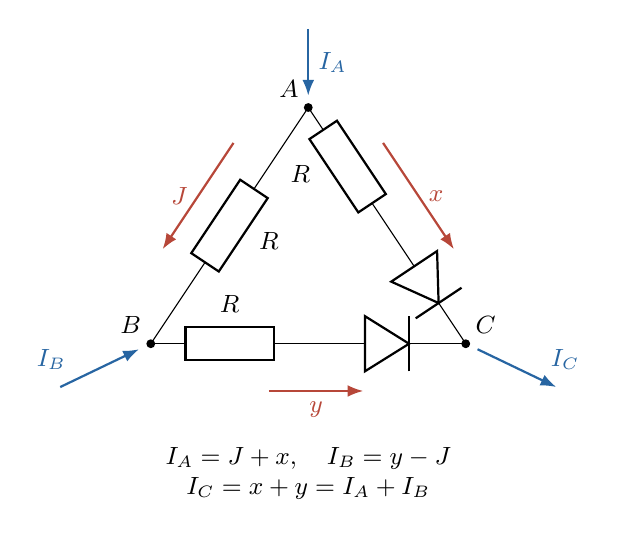
\begin{tikzpicture}
 \draw(0,3)to[R](-2,0);
 \draw(0,3)to[R](1,1.5)to[D](2,0);
 \draw(-2,0)to[R](0,0)to[D](2,0);
 \node at(-.5,1.3){$R$};
 \node at(-.1,2.15){$R$};
 \node at(-1,.5){$R$};
 \ports
 \draw[red,vec](-.95,2.55)--(-1.85,1.2)node[midway,left]{$J$};
 \draw[red,vec](.95,2.55)--(1.85,1.2)node[midway,right]{$x$};
 \draw[red,vec](-.5,-.6)--(.7,-.6)node[midway,below]{$y$};
 \node[align=center]at(0,-1.65){$I_A=J+x,\quad I_B=y-J$\\$I_C=x+y=I_A+I_B$};
\end{tikzpicture}
\begin{tikzpicture}[scale=1.05]
 \path[fill=gray!13](-3,3)--(-3,-3)--(3,-3)--cycle;
 \path[fill=blue!10](-1.5,3)--(3,3)--(3,-1.5)--(0,0)--cycle;
 \path[fill=orange!16](-3,3)--(-1.5,3)--(0,0)--cycle;
 \path[fill=green!13](0,0)--(3,-1.5)--(3,-3)--cycle;
 \draw[gray,vec](-3.35,0)--(3.45,0)node[right]{$I_A$};
 \draw[gray,vec](0,-3.35)--(0,3.5)node[above]{$I_B$};
 \draw[thick](-3,3)--(3,-3);
 \draw[blue,thick](-1.5,3)--(0,0)--(3,-1.5);
 \node[blue]at(1.55,1.75){I};
 \node[orange!70!black]at(-1.65,2.55){II};
 \node[green!40!black]at(2.5,-1.85){III};
 \node[align=center]at(-1.5,-1.75){$I_A+I_B<0$\\无稳态解};
 \node[below left]at(0,0){$O$};
 \node[above]at(-1.5,3){$2I_A+I_B=0$};
 \node[right,align=left]at(3,-1.5){$I_A+2I_B=0$};
 \node[right,align=left]at(3,-3){$I_A+I_B=0$};
 \node[anchor=north,align=left]at(.2,-3.65){
 I：两支路导通；II：$A\to C$ 截止；III：$B\to C$ 截止。\\
 斜线 $I_A+I_B=0$ 上两二极管电流均为零，电势一般不唯一。};
\end{tikzpicture}
\end{document}
